\documentclass[tikz,border=6pt]{standalone}
% Shared look for the Details diagrams: the site's cave palette on a
% transparent ground, so the SVG sits on the dark page with no box around it.
\usepackage[T1]{fontenc}
\usepackage{helvet}
\usepackage{amsmath,amssymb}
\renewcommand{\familydefault}{\sfdefault}
\usetikzlibrary{arrows.meta,positioning,calc,backgrounds,fit}
\definecolor{ink}{HTML}{D7DBE0}
\definecolor{dim}{HTML}{99A1AD}
\definecolor{faint}{HTML}{6D7682}
\definecolor{rock}{HTML}{21262E}
\definecolor{edge}{HTML}{4A525E}
\definecolor{lamp}{HTML}{7AA2F7}
\definecolor{gold}{HTML}{F5B301}
\definecolor{moss}{HTML}{4AA06A}
\definecolor{ember}{HTML}{E05A4D}
\tikzset{
  every node/.style={text=ink},
  flow/.style={-{Stealth[length=2.4mm]}, line width=0.8pt, draw=dim},
  call/.style={-{Stealth[length=2mm]}, line width=0.7pt, draw=gold, dashed},
  lab/.style={font=\scriptsize, text=dim, align=center, inner sep=1.5pt},
}

\begin{document}
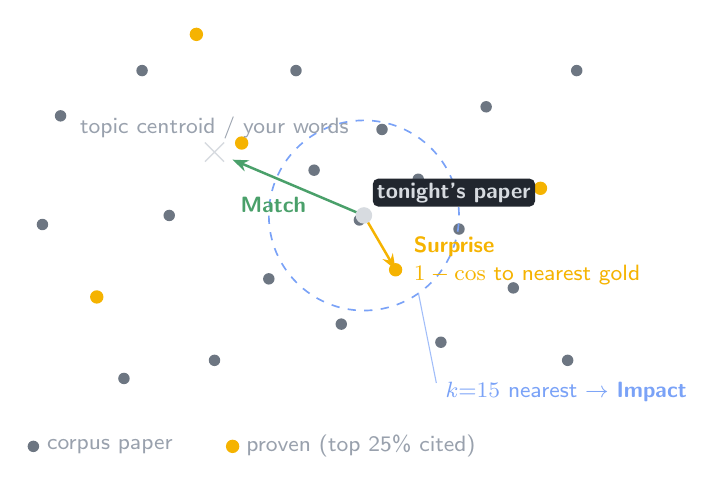
\begin{tikzpicture}[scale=1.15, lab/.append style={font=\footnotesize}]
% corpus papers: grey dots, gold when proven (citation pct >= 0.75)
\foreach \x/\y/\p in {
  -2.6/1.4/0, -2.2/-0.6/1, -1.7/1.9/0, -1.4/0.3/0, -0.9/-1.3/0, -0.6/1.1/1,
  -0.3/-0.4/0, 0.2/0.8/0, 0.5/-0.9/0, 0.7/0.25/0, 0.95/1.25/0, 1.1/-0.3/1,
  1.35/0.7/0, 1.6/-1.1/0, 1.8/0.15/0, 2.1/1.5/0, 2.4/-0.5/0, 2.7/0.6/1,
  -1.9/-1.5/0, -2.8/0.2/0, 3.0/-1.3/0, 0.0/1.9/0, -1.1/2.3/1, 3.1/1.9/0} {
  \ifnum\p=1 \fill[gold] (\x,\y) circle (2.1pt); \else \fill[faint] (\x,\y) circle (1.8pt); \fi
}
% the candidate
\coordinate (c) at (0.75,0.3);
% its k nearest neighbours
\draw[lamp, line width=0.6pt, dashed] (c) circle (1.05);
\node[lab, text=lamp, anchor=west] at (1.6,-1.65) {$k{=}15$ nearest $\to$ \textbf{Impact}};
\draw[lamp!70, line width=0.4pt] (1.55,-1.55) -- ($(c)+(-55:1.05)$);
% nearest proven paper
\coordinate (pr) at (1.1,-0.3);
\draw[gold, line width=0.9pt, -{Stealth[length=2mm]}] (c) -- (pr);
\node[lab, text=gold, anchor=west] at (1.25,-0.05) {\textbf{Surprise}};
\node[lab, text=gold, anchor=west] at (1.25,-0.36) {$1-\cos$ to nearest gold};
% topic centroid / touchstone
\coordinate (t) at (-0.9,1.0);
\draw[ink, line width=0.5pt] (t) +(-3pt,-3pt) -- +(3pt,3pt) (t) +(-3pt,3pt) -- +(3pt,-3pt);
\draw[moss, line width=0.9pt, -{Stealth[length=2mm]}] (c) -- ($(t)!0.12!(c)$);
\node[lab, anchor=south] at (t) [yshift=3pt] {topic centroid / your words};
\node[lab, text=moss] at (-0.25,0.42) {\textbf{Match}};
\fill[ink] (c) circle (2.6pt);
\node[lab, text=ink, anchor=south west, fill=rock, rounded corners=2pt] at (c) [xshift=3pt, yshift=3pt] {\textbf{tonight's paper}};
% legend
\fill[faint] (-2.9,-2.25) circle (1.8pt); \node[lab, anchor=west] at (-2.8,-2.25) {corpus paper};
\fill[gold] (-0.7,-2.25) circle (2.1pt); \node[lab, anchor=west] at (-0.6,-2.25) {proven (top 25\% cited)};
\end{tikzpicture}
\end{document}
